\documentclass[a4paper,10pt]{article}
\usepackage[left=1cm,right=1cm,top=1.50cm,bottom=1.50cm]{geometry}
\usepackage{physics}
\usepackage[UTF8]{ctex}
\usepackage{float}
\usepackage{graphicx}
\usepackage{siunitx}
\begin{document}
\section{Formalism}
\paragraph{Operators}
\begin{align*}
     & \bra{x}\hat{P}\ket{\psi}=-i\hbar\pdv{\psi(x)}{x}                                                                                   \\
     & \bra{p}\hat{X}\ket{\psi}=i\hbar\pdv{\varphi(p)}{p}                                                                                 \\
     & \comm{A}{BC}=B\comm{A}{C}+\comm{A}{B}C\qq{}\comm{AB}{C}=A\comm{B}{C}+\comm{A}{C}B                                                  \\
     & \comm{\hat{X}}{\hat{P}}=i\hbar\qq{}\comm{\hat{X}}{\hat{H}}=\frac{i\hbar\hat{P}}{m}\qq{}\comm{\hat{P}}{\hat{H}}=-i\hbar\dv{V(X)}{X} \\
     & \bra{x}\hat{H}\ket{\psi}=-\frac{\hbar^2}{2m}\pdv[2]{\psi(x)}{x}+V(x)\psi(x)
\end{align*}
\paragraph{Expectation Value}
$$\expval{\hat{A}}_{\ket{\psi}}=\bra{\psi}\hat{A}\ket{\psi}$$
$$\expval{\hat{X}^2}_{\ket{\psi}}=\int_{-\infty}^{\infty}x^2\psi^\ast(x)^2\psi(x)\dd{x}$$
$$\expval{\hat{P}}_{\ket{\psi}}=\int_{-\infty}^{\infty}\psi^\ast(x)\left(-i\hbar\pdv{\psi(x)}{x}\right)\dd{x}$$
$$\expval{\hat{P}^2}_{\ket{\psi}}=\int_{-\infty}^{\infty}\psi^\ast(x)\left(-\hbar^2\pdv[2]{\psi(x)}{x}\right)\dd{x}$$
\paragraph{Complete Set of Commutable Observables}
Suppose $A,B$ hermite and $\comm{A}{B}=0$.
\begin{itemize}
    \item There exists (at least) a basis of common eigenvectors that diagonalize them both.
    \item It is possible to construct an orthonormal basis of the state space by the eigenstates that are common to both observables, i.e. $A\ket{\psi_i}=a\ket{\psi_i}$ and $B\ket{\psi_i}=b\ket{\psi_i}$.
\end{itemize}
对于简并的情况,$A$对应某一特征值的特征空间中特征向量的线性组合,可以构造为$B$的特征向量。

C.S.C.O.是指对单独一个物理量$\hat{A}$,由于简并,测量其特征值并不能确定态矢量,需要测量另外一个甚至多个物理量$\hat{B},\hat{C}$,通过测量结果$(a,b,c)$来从多种可能组合中确定唯一的本征态矢量。

C.S.C.O. would have following properties:
\begin{itemize}
    \item All observables commute by pair.
    \item Specifying the eigenvalues (from the measurement) would uniquely determine a common eigenstate.
\end{itemize}
\paragraph{Momentum and Position}
Konwing the position representation, we can find out the momentum representation and vice versa.
$$p(x)=\bra{x}\ket{p}=\frac{1}{\sqrt{2\pi\hbar}}e^{ipx/\hbar}\qq{the constant factor is to satisfy orthonormal condition}\bra{p^\prime}\ket{p}=\delta(p^\prime-p)$$
$$x(p)=\bra{p}\ket{x}=\frac{1}{\sqrt{2\pi\hbar}}e^{-ipx/\hbar}$$
Any state $\ket{\psi}$ can be expressed in both representations:
$$\psi(x)=\bra{x}\ket{\psi}=\int_{-\infty}^{\infty}\bra{x}\ket{p}\bra{p}\ket{\psi}\dd{p}=\frac{1}{\sqrt{2\pi\hbar}}\int_{-\infty}^{\infty}e^{ipx/\hbar}\varphi(p)\dd{p}$$
$$\varphi(p)=\bra{p}\ket{\psi}=\int_{-\infty}^{\infty}\bra{p}\ket{x}\bra{x}\ket{\psi}\dd{x}=\frac{1}{\sqrt{2\pi\hbar}}\int_{-\infty}^{\infty}e^{-ipx/\hbar}\psi(x)\dd{x}$$
Thy are releated by Fourier Transform:
$$k=\frac{p}{\hbar}\qq{then:}$$
$$\psi(x)=\frac{1}{\sqrt{2\pi}}\int_{-\infty}^{\infty}g(k)e^{ikx}\dd{k}$$
$$g(k)=\frac{1}{\sqrt{2\pi}}\int_{-\infty}^{\infty}\psi(x)e^{-ikx}\dd{x}$$
Time evolution of wave function:
$$\psi(x,t)=\frac{1}{\sqrt{2\pi}}\int_{-\infty}^{\infty}g(k)e^{i(kx-\omega t)}\dd{k},\omega=\frac{\hbar k^2}{2m}$$
\section{Schrödinger Equation}
$$i\hbar\pdv{t}\ket{\Psi(t)}=\hat{H}\ket{\Psi(t)}$$
$$\hat{H}\ket{\psi}=E\ket{\psi}$$
$$i\hbar\pdv{\psi(x,y,z,t)}{t}=\left(-\frac{\hbar^2}{2m}\laplacian+V(x,y,z)\right)\psi(x,y,z,t)$$
$$-iE/\hbar\ket{\psi}=\pdv{t}\ket{\psi}\Rightarrow\ket{\psi,t}=\ket{\psi,0}e^{-iEt/\hbar}$$
\paragraph{Ehrenfest's Theorem}
$$\dv{t}\expval{\hat{A}}_{\ket{\psi}}=\frac{1}{i\hbar}\expval{[\hat{A},\hat{H}]}_{\ket{\psi}}$$
\section{1-D Potential Problem}
The general steps of solving 1-D potential well problem is to first solve the time independent Schrödinger equation in each region, then apply boundary conditions to determine the coefficients of the wave function.

Also, In some cases, the initial state is not an eigenstate of the Hamiltonian, then we can expand it in terms of eigenstates by Fourier Transform or Fourier Series.
\paragraph{General Properties of Wave Function}
\begin{itemize}
    \item wave function solutions to Schrödinger equation need single valued continuous.
    \item solutions should be normalizable, at least for bound states.
    \item if potential possesses space symmetry, i.e. $V(x)=V(-x)$, then the wave function should be either even or odd.
\end{itemize}
\paragraph{Free Particle}
A particle in free space means that $V(x)=0$ everywhere.
$$\qq{In x representation is}\bra{x}\ket{p,t}=e^{-iEt/\hbar}\bra{x}\ket{p}=\frac{1}{\sqrt{2\pi\hbar}}e^{i(kx-\omega t)}$$
$$\qq{where}k=\frac{p}{\hbar},\omega=\frac{E}{\hbar}=\frac{\hbar k^2}{2m}$$
$$\qq{phase velocity}v_p=\frac{\omega}{k}=\frac{\hbar k}{2m}=\frac{p}{2m}$$
$$\qq{group velocity}v_g=\dv{\omega}{k}=\frac{\hbar k}{m}=\frac{p}{m}$$
\paragraph{Infinite Potential Well}
$$V(x)=\begin{cases}
        0      & 0<x<a                  \\
        \infty & \text{everywhere else}
    \end{cases}$$
Its solution is $\psi(x)=C\cos(kx)+D\sin(kx)$, where $k=\sqrt{2mE}/\hbar$. Considering boundary condition, $C=0,k=\frac{n\pi}{a}$.
$$E_n=\frac{n^2\pi^2\hbar^2}{2ma^2}=\frac{\hbar^2k_n^2}{2m}$$
$$\psi_n(x)=\sqrt{\frac{2}{a}}\sin\left(\frac{n\pi x}{a}\right)$$
$$\Psi_n(x,t)=\sqrt{\frac{2}{a}}\sin\left(\frac{n\pi x}{a}\right)e^{-iE_nt/\hbar}$$
$$\qq{They are mutually orthogonal}\int\psi_n^\ast(x)\psi_m(x)\dd{x}=\delta_{nm}$$
\paragraph{Potential Step}
$$V(x)=\begin{cases}
        0   & x<0\qq{region I}  \\
        V_0 & x>0\qq{region II}
    \end{cases}$$
\subparagraph{Case $E>V_0$}
$$\psi_1(x)=Ae^{ik_1x}+Be^{-ik_1x}\qq{for region I where}k_1=\sqrt{2mE}/\hbar$$
$$\psi_2(x)=Ce^{ik_2x}+De^{-ik_2x}\qq{for region II where}k_2=\sqrt{2m(E-V_0)}/\hbar$$
Apply boundary condition at $x=0$:
$$\mqty(1&1\\k_1&-k_1)\mqty(A\\B)=\mqty(1&1\\k_2&-k_2)\mqty(C\\D)$$
Define M matrix and S matrix:
$$\mqty(C\\D)=M\mqty(A\\B)\qq{M is called transfer matrix}M=\frac{1}{2k_2}\mqty(k_{1}+k_{2}&k_{2}-k_{1}\\k_{2}-k_{1}&k_{1}+k_{2})$$
$$\mqty(B\\C)=S\mqty(A\\D)\qq{S is called scattering matrix}S=\frac{1}{k_1+k_2}\mqty(k_{1}-k_{2}&2k_{2}\\2k_{1}&k_{2}-k_{1})$$
Their relation is:
$$M=\frac{1}{S_{12}}\mqty(-\det S&S_{22}\\-S_{11}&1)$$
$$S=\frac{1}{M_{22}}\mqty(-M_{21}&1\\\det M&M_{12})$$
$$R=\frac{j_{ref}}{j_{ini}}=\abs{\frac{B}{A}}^2\qq{reflection ratio}$$
$$T=\frac{j_{tran}}{j_{ini}}=\frac{k_2}{k_1}\abs{\frac{C}{A}}^2\qq{transmission ratio}$$
When initially we only have waves travelling towards right, then $D=0$.
$$\frac{B}{A}=\frac{k_1-k_2}{k_1+k_2},\frac{C}{A}=\frac{2k_1}{k_1+k_2}$$
\subparagraph{Probability Current in Quantum}
The local conservation of charge is expressed as:
$$\pdv{\rho(r,t)}{t}+\div\va{j}(r,t)=0$$
In Quantum Mechanics, the total probability $\bra{\psi}\ket{\psi}$ is conserved, and the local probability density is $\rho(x,t)=\psi^\ast\psi$.
For wave function satisfying Schrödinger Equation, we can define a probability current so that the local conservation is satisfied.

Its regorous definition is:
$$\va{j}(x,t)=\frac{\hbar}{2mi}\left(\psi^\ast\grad\psi-\psi\grad\psi^\ast\right)$$
For a plane wave type $\psi(x,t)=Ae^{i(kx-\omega t)}$, the probability current is:
$$j(x,t)=\abs{A}^2\frac{\hbar k}{m}\qq{which is analogous to the intensity in EM wave}$$
\subparagraph{Case $E<V_0$}
$$\psi_1(x)=Ae^{ik_1x}+Be^{-ik_1x}\qq{for region I where}k_1=\sqrt{2mE}/\hbar$$
$$\psi_2(x)=De^{-k_2^\prime x}\qq{C has to be 0 for region II where}k_2^\prime=\sqrt{2m(V_0-E)}/\hbar$$
Apply boundary condition at $x=0$:
\begin{align*}
     & A+B=D\qq{and}ik_1(A-B)=-k_2^\prime D                                                                    \\
     & \frac{B}{A}=\frac{k_1-ik_2}{k_1+ik_2},\frac{D}{A}=\frac{2k_1}{k_1+ik_2}                                 \\
     & \qq{There will be total reflection, i.e.}R=\abs{\frac{B}{A}}^2=1,T=\frac{k_2}{k_1}\abs{\frac{C}{A}}^2=0
\end{align*}
\paragraph{Potential Barrier}
$$V(x)=\begin{cases}
        V_0 & 0<x<a                  \\
        0   & \text{everywhere else}
    \end{cases}$$
\subparagraph{Case $E>V_0$}
\begin{align*}
    \psi_1(x) & =Ae^{ik_1x}+Be^{-ik_1x}\qq{for region I where}k_1=\sqrt{2mE}/\hbar        \\
    \psi_2(x) & =Ce^{ik_2x}+De^{-ik_2x}\qq{for region II where}k_2=\sqrt{2m(E-V_0)}/\hbar \\
    \psi_3(x) & =Fe^{ik_1x}+Ge^{-ik_1x}\qq{for region III}
\end{align*}
Apply boundary condition at $x=0$ and $x=a$:
\begin{align*}
    A+B                         & =C+D                         \\
    k_1(A-B)                    & =k_2(C-D)                    \\
    Ce^{ik_2a}+De^{-ik_2a}      & =Fe^{ik_1a}+Ge^{-ik_1a}      \\
    k_2(Ce^{ik_2a}-De^{-ik_2a}) & =k_1(Fe^{ik_1a}-Ge^{-ik_1a})
\end{align*}
The strategy is to eliminate $C$ and $D$ to get relation between $A,B$ and $F,G$.
\begin{align*}
    \frac{F}{A} & =\frac{4k_1k_2e^{-ik_1a}}{4k_1k_2\cos(k_2a)-2i(k_1^2+k_2^2)\sin(k_2a)}                                                                                                            \\
    T           & =\frac{k_1}{k_1}\abs{\frac{F}{A}}^2=\frac{4k_1^2k_2^2}{4k_1^2k_2^2+(k_1^2-k_2^2)^2\sin^2(k_2a)}=1/\left(1+\frac{1}{4}\left(\frac{k_1^2-k_2^2}{k_1k_2}\right)^2\sin^2(k_2a)\right) \\
    R           & =\abs{\frac{B}{A}}^2=1-T=\frac{(k_1^2-k_2^2)^2\sin^2(k_2)}{4k_1^2k_2^2+(k_1^2-k_2^2)^2\sin^2(k_2a)}                                                                               \\
                & \qq{Since} \left(\frac{k_1^2-k_2^2}{k_1k_2}\right)^2=\frac{V_0^2}{E(E-V_0)}=\frac{1}{\varepsilon(\varepsilon-1)}\qq{as}\varepsilon=\frac{E}{V_0}                                  \\
    T           & =\frac{1}{1+\frac{1}{4\varepsilon(\varepsilon-1)}\sin^2(k_2a)}\qq{is maximum (equals 1) whenever}k_2a=m\pi,m=1,2,3,\cdots                                                         \\
    R           & =\frac{\sin^2(k_2a)}{4\varepsilon(\varepsilon-1)+\sin^2(k_2a)}
\end{align*}
\subparagraph{Case $E<V_0$}
\begin{align*}
    \psi_1(x) & =Ae^{ik_1x}+Be^{-ik_1x}\qq{for region I where}k_1=\sqrt{2mE}/\hbar                             \\
    \psi_2(x) & =Ce^{k_2^\prime x}+De^{-k_2^\prime x}\qq{for region II where}k_2^\prime=\sqrt{2m(V_0-E)}/\hbar \\
    \psi_3(x) & =Fe^{ik_1x}+Ge^{-ik_1x}\qq{for region III}
\end{align*}
Replace all the $k_2$ by $ik_2^\prime$ in previous calculation, we get:
\begin{align*}
    \frac{F}{A} & =\frac{e^{-ik_1a}}{\cosh(k_2^\prime a)+\frac{i({k_2^\prime}^2-k_1^2)}{2k_1k_2}\sinh(k_2^\prime a)}                                                          \\
    T           & =\abs{\frac{F}{A}}^2=\frac{1}{\cosh^2(k_2^\prime a)+\frac{({k_2^\prime}^2-k_1^2)^2}{4k_1^2{k_2^\prime}^2}\sinh^2(k_2^\prime a)}                             \\
                & \qq{Since} \left(\frac{k_1^2-k_2^2}{k_1k_2}\right)^2=\frac{V_0^2}{E(E-V_0)}=\frac{1}{\varepsilon(\varepsilon-1)}\qq{as}\varepsilon=\frac{E}{V_0}            \\
    T           & =\frac{1}{1+\frac{1}{4\varepsilon(\varepsilon-1)}\sinh^2(k_2^\prime a)}                                                                                     \\
    T           & \approx 16\varepsilon(1-\varepsilon)e^{-2k_2^\prime a}\qq{as $a$ gets large, i.e.}k_2^\prime>1\qq{thus}\sinh(k_2^\prime a)\approx\frac{e^{k_2^\prime a}}{2} \\
    a_0         & =\frac{1}{k_2^\prime}=\frac{\hbar}{\sqrt{2m(V_0-E)}}\qq{threshold for width of barrier}                                                                     \\
\end{align*}
\paragraph{Finite Potential Well}
$$V(x)=\begin{cases}
        -V_0 & \text{for}-a<x<a       \\
        0    & \text{everywhere else}
    \end{cases}$$
\subparagraph{Bound Case $-V_0<E<0$}
General solution is:
\begin{align*}
    \psi_1(x) & =Ae^{k_1x}\qq{for region I where}k_1=\sqrt{2m(-E)}/\hbar                   \\
    \psi_2(x) & =C\sin(k_2x)+D\cos(k_2x)\qq{for region II where}k_2=\sqrt{2m(V_0+E)}/\hbar \\
    \psi_3(x) & =Ge^{-k_1x}\qq{for region III}
\end{align*}
Exploit the requirement on the odd and evenness of the wave function here to simplify.
\begin{align*}
    \qq{Even solution:} &                                                                                                       \\
    \psi_1              & =Ae^{k_1x},\psi_2=D\cos(k_2x),\psi_3=Ae^{-k_1x}                                                       \\
                        & \qq{which satisfies} D\cos(k_2a)=Ae^{-k_1a},k_2D\sin(k_2a)=k_1Ae^{-k_1a}\Rightarrow k_2\tan(k_2a)=k_1 \\
    \tan z              & =\sqrt{\frac{z_0^2}{z^2}-1}\qq{where}z=k_2a,z_0=\frac{a\sqrt{2mV_0}}{\hbar}                           \\
    \qq{Odd solution:}  &                                                                                                       \\
    -\cot z             & =\sqrt{\frac{z_0^2}{z^2}-1}\qq{where}z=k_2a,z_0=\frac{a\sqrt{2mV_0}}{\hbar}                           \\
\end{align*}
One has to plot a graph to find the solution, the intersection of $\tan z$ or $-\cot z$ and $\sqrt{\frac{z_0^2}{z^2}-1}$ gives $k_2$, then $E$. The results is quantized.
\subparagraph{Scattering Case $E>0$}
This problem is already solved in the "Potential Barrier" part, just take care with $k_2,2a$.
\begin{align*}
    T       & =\frac{1}{1+\frac{1}{4\varepsilon(\varepsilon+1)}\sin^2(2k_2a)}\qq{where}\varepsilon=\frac{E}{V_0} \\
    k_2(2a) & =m\pi\qq{resonance condition for the maximum $T$}
\end{align*}
\begin{figure}[H]
    \centering
    \begin{minipage}[t]{0.5\linewidth}
        \centering
        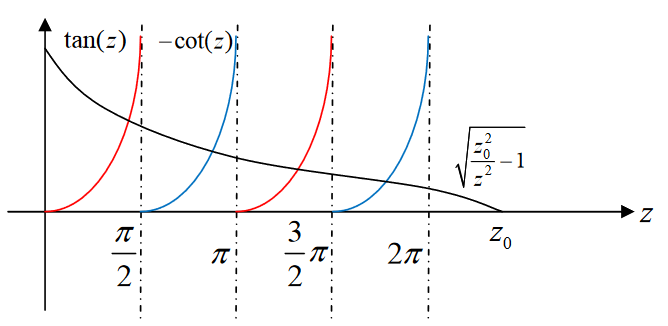
\includegraphics[width=0.95\linewidth]{finite-potential-solution.png}
        \caption{Finite Potential Well}
    \end{minipage}%
    \begin{minipage}[t]{0.5\linewidth}
        \centering
        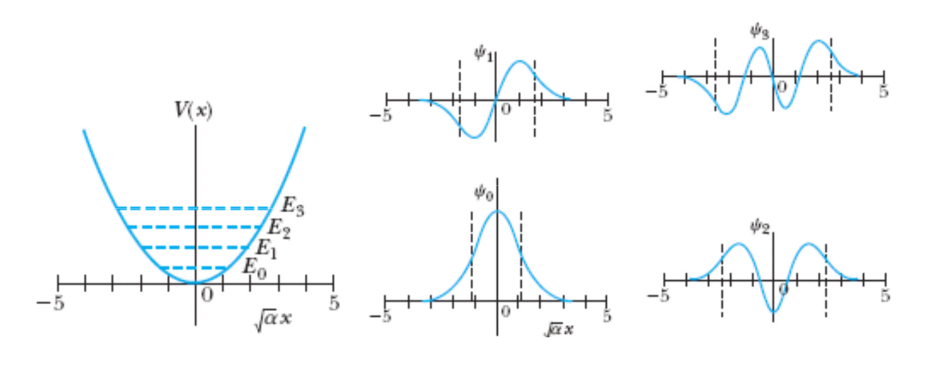
\includegraphics[width=0.95\linewidth]{harmonic-oscillator-solution.png}
        \caption{Harmonic Oscillator}
    \end{minipage}
\end{figure}
\paragraph{Harmonic Oscillator}
\subparagraph{Derivation}
The quantum problem is to solve the Schrödinger Equation for the Potential $V(x)=\frac{1}{2}kx^2$.
\begin{align*}
    \qq{Time independent Schrödinger Equation} & \left(-\frac{\hbar^2}{2m}\dv[2]{x}+\frac{1}{2}kx^2\right)\psi=E\psi             \\
    \qq{Cosmetic}                              & \omega^2=\frac{k}{m},K=\frac{2E}{\hbar\omega},\xi=x\sqrt{\frac{m\omega}{\hbar}} \\
    \Longrightarrow                            & \dv[2]{\psi}{\xi}+(K-\xi^2)\psi=0
\end{align*}
Guess work:
$$\psi(\xi)=h(\xi)e^{-\xi^2/2} \qq{where $h(\xi)$ is an even or odd polynomial of $\xi$ whose coefficients need to be determined}$$
\begin{align*}
    h(\xi)=\xi^p\sum_{m=0}^{\infty}a_{2m}\xi^{2m}\qq{$p$ can either be 0 or 1 corresponding to even or odd series}
\end{align*}
Throw the form of $\psi(\xi)$ into the Schrödinger Equation and solve for $a_{2m}$:
\begin{align*}
     & \dv[2]{h}{\xi}-2\xi\dv{h}{\xi}+(K-1)h=0             \\
     & a_{2m+2}=\frac{2(2m+p)+1-K}{(2m+p+2)(2m+p+1)}a_{2m}
\end{align*}
If $h(\xi)$ has infinite terms, then it's goging to contradict with the normalization condition. So the series must terminate at some point:
\begin{align*}
    K       & =2(2m_0+p)+1=2n+1\qq{where $n=2m_0+p$}                             \\
    E_n     & =(n+\frac{1}{2})\hbar\omega,n=0,1,2,\cdots                         \\
    a_{j+2} & =\frac{-2(n-j)}{(j+1)(j+2)}a_j\qq{where $n,j$ is both even or odd}
\end{align*}
\subparagraph{Determine the Wave Function}Generally, for given $n$, one has to throw into the recursion relation and normalize the wave function.
\begin{align*}
    H_0    & =1\qq{} H_1=2\xi\qq{}H_2=4\xi^2-2                                                                      \\
    H_3    & =8\xi^3-12\xi\qq{} H_4=16\xi^4-48\xi^2+12\qq{}H_5=32\xi^5-160\xi^3+120\xi                              \\
    H_n(x) & =(-1)^ne^{x^2}\dv[n]{x}e^{-x^2}                                                                        \\
    \Psi_n & =\left(\frac{m\omega}{\pi\hbar}\right)^{\frac{1}{4}}\frac{1}{\sqrt{2^nn!}}H_n(\xi)e^{\frac{-\xi^2}{2}}
\end{align*}
\section{Hydrogen Atom}
Hydrogen Atom is the only atomic element which has a single electron and thus simplest Hamiltonian and has rigorous analytic solution in quantum.
\paragraph{Schrödinger Equation}
Using center of mass frame, the Hamiltonian will decompose into the free-particle motion of the total mass, and relative motion of reduced mass.

The Hamiltonian of relative motion is:
$$H_{total}=-\frac{\hbar^2}{2m}\laplacian+V(r)\qq{where} V(r)=-\frac{e^2}{4\pi\epsilon_0r},m=\frac{m_eM}{m_e+M_n}$$
since $V(r)$ is spherically symmetric, the Schrödinger Equation can be solved in spherical coordinate:
\begin{align*}
    \laplacian                          & =\pdv[2]{x}+\pdv[2]{y}+\pdv[2]{z}                                                                                                                                                                            \\
                                        & =\frac{1}{r^2}\pdv{r}\left(r^2\pdv{r}\right)+\frac{1}{r^2\sin\theta}\pdv{\theta}\left(\sin\theta\pdv{\theta}\right)+\frac{1}{r^2\sin^2\theta}\pdv[2]{\phi}                                                   \\
                                        & =\frac{1}{r}\pdv[2]{r}r+\frac{1}{r^2}\Lambda^2                                                                                                                                                               \\
    \qq{Schrödinger Equation}           & -\frac{\hbar^2}{2m}\left(\frac{1}{r^2}\pdv{r}\left(r^2\pdv{r}\right)+\frac{1}{r^2\sin\theta}\pdv{\theta}\left(\sin\theta\pdv{\theta}\right)+\frac{1}{r^2\sin^2\theta}\pdv[2]{\phi}\right)\psi+V(r)\psi=E\psi \\
    \qq{Wave function can be separated} & \psi(r,\theta,\phi)=R(r)Y(\theta,\phi)=R(r)\Theta(\theta)\Phi(\phi)                                                                                                                                          \\
    \frac{1}{R}\dv{r}(r^2\dv{R}{r})     & -\frac{2mr^2}{\hbar^2}\left(V(r)-E\right)=l(l+1)=-\frac{1}{Y}\left(\frac{1}{\sin\theta}\pdv{\theta}(\sin\theta\pdv{Y}{\theta})+\frac{1}{\sin^2\theta}\pdv[2]{Y}{\phi}\right)
\end{align*}
These are the two differential equations need to be solved.
\paragraph{Angular Part}
\begin{align*}
                                   & \frac{1}{\Theta}\left(\sin\theta\dv{\theta}(\sin\theta\dv{\Theta}{\theta})\right)+l(l+1)\sin^2\theta=m^2=-\frac{1}{\Phi}\dv[2]{\Phi}{\phi} \\
    \qq{general form of $\Phi$:}   & \Phi(\phi)=e^{im\phi}                                                                                                                      \\
    m=0,\pm1,\pm2,\cdots           & \qq{since}\Phi(\phi+2\pi)=\Phi(\phi)                                                                                                       \\
    \qq{general form of $\Theta$:} & \Theta(\theta)=AP_l^m(\cos\theta)\qq{$A$ is a factor determined by normalization}                                                          \\
    P_l^m(x)                       & =(1-x^2)^{\frac{\abs{m}}{2}}\dv[\abs{m}]{x}P_l(x)\qq{$P_l^m(x)$ is called associated Legendre function}                                    \\
    P_l(x)                         & \equiv\frac{1}{2^ll!}\dv[l]{x}(x^2-1)^l\qq{the Legendre Polynomial}
\end{align*}
For orbit angular momentum:
\begin{align*}
     & \hat{L}^2Y(\theta,\phi)=l(l+1)\hbar^2Y(\theta,\phi)\qq{and}\hat{L}^2=-\hat{\Lambda}^2\hbar^2 \\
     & \Lambda^2Y(\theta,\phi)=l(l+1)Y(\theta,\phi)\qq{then make substitution}                      \\
     & \hat{L_Z}=-i\hbar\pdv{\phi}\qq{and}\hat{L_Z}Y(\theta,\phi)=m\hbar Y(\theta,\phi)
\end{align*}
Expressions of Legendre Polynomials:
\begin{align*}
     & P_0(x)=1, P_1(x)=x, P_2(x)=\frac{1}{2}(3x^2-1)                                                                                                       \\
     & P_3(x)=\frac{1}{2}(5x^3-3x),P_4(x)=\frac{1}{8}(35x^4-30x^2+3), P_5(x)=\frac{1}{8}(63x^5-70x^3+15x)                                                   \\
     & P_0^0=1                                                                                                                                              \\
     & P_1^1=\sin\theta,P_1^0=\cos\theta                                                                                                                    \\
     & P_2^2=3\sin^2\theta,P_2^1=3\sin\theta\cos\theta,   P_2^0=\frac{1}{2}(3\cos^2\theta-1)                                                                \\
     & P_3^3=15\sin^3\theta,  P_3^2=15\sin^2\theta\cos\theta,  P_3^1=\frac{3}{2}\sin\theta(5\cos^2\theta-1),   P_3^0=\frac{1}{2}(5\cos^3\theta-3\cos\theta) \\
\end{align*}
Now $Y(\theta,\phi)$ is expressed as $Y_l^m(\theta,\phi)$, the spherical harmonics (eigenfunction for the orbital angular momentum), and the Legendre polynomial is meaningful when $l=0,1,2,\cdots$ and $m=-l,-l+1,\cdots,l-1,l$.
In the angular momentum theory, $\abs{L}=\sqrt{l(l+1)}\hbar$ and $L_z=m\hbar$.
\begin{align*}
     & \int_0^{\pi}\dd{\theta}\int_0^{2\pi}\dd{\phi}\abs{Y_l^m}^2\sin\theta=1                                                                                                                                                                                                                      \\
     & \qq{which is normalization condition over angular part}                                                                                                                                                                                                                                     \\
     & Y_0^0=\left(\frac{1}{\sqrt{4\pi}}\right)^\frac{1}{2}                                                                                                                                                                                                                                        \\
     & Y_1^0=\left(\frac{3}{4\pi}\right)^\frac{1}{2}\cos\theta, Y_1^{\pm1}=\mp\left(\frac{3}{8\pi}\right)^\frac{1}{2}\sin\theta e^{\pm i\phi}                                                                                                                                                      \\
     & Y_2^0=\left(\frac{5}{16\pi}\right)^\frac{1}{2}\left(3\cos^2\theta-1\right), Y_2^{\pm1}=\mp\left(\frac{15}{8\pi}\right)^\frac{1}{2}\sin\theta\cos\theta e^{\pm i\phi}, Y_2^{\pm2}=\left(\frac{15}{32\pi}\right)^\frac{1}{2}\sin^2\theta e^{\pm2i\phi}                                        \\
     & Y_3^0=\left(\frac{7}{16\pi}\right)^\frac{1}{2}\left(5\cos^3\theta-3\cos\theta\right), Y_3^{\pm1}=\mp\left(\frac{21}{64\pi}\right)^\frac{1}{2}\sin\theta\left(5\cos^2\theta-1\right)e^{\pm i\phi}, Y_3^{\pm2}=\left(\frac{105}{32\pi}\right)^\frac{1}{2}\sin^2\theta\cos\theta e^{\pm2i\phi} \\
     & Y_3^{\pm3}=\mp\left(\frac{35}{64\pi}\right)^\frac{1}{2}\sin^3\theta e^{\pm3i\phi}                                                                                                                                                                                                           \\
     & Y_l^m(\theta,\phi)=\epsilon\sqrt{\frac{(2l+1)(l-\abs{m})!}{4\pi(l+\abs{m})!}}P_l^{m}(\cos\theta)e^{im\phi}\qq{general formula for spherical harmonics}                                                                                                                                      \\
     & \int_0^{\pi}\dd{\theta}\int_0^{2\pi}\dd{\phi}{Y_{l^\prime}^{m^\prime}}^\ast Y_l^m\sin\theta=\delta_{ll^\prime}\delta_{mm^\prime}\qq{eigenfunctions for Hermitian operator $\hat{L}$ must be orthogonal}
\end{align*}
\paragraph{Radial Part}
\begin{align*}
    \qq{define a function}      & u(r)=rR(r)                                                                                                                                                            \\
                                & -\frac{\hbar^2}{2m}\dv[2]{u}{r}+\left(V(r)+\frac{\hbar^2}{2m}\frac{l(l+1)}{r^2}\right)u=Eu                                                                            \\
    \qq{effective potential is} & V_{eff}=V+\frac{l(l+1)\hbar^2}{2mr^2}\qq{analogous to classical, angular momentum is}\sqrt{l(l+1)\hbar}                                                               \\
    \dv[2]{u}{\rho}             & =\left(1-\frac{\rho_0}{\rho}+\frac{l(l+1)\hbar^2}{\rho^2}\right)u\qq{with substitution}k=\frac{\sqrt{-2mE}}{\hbar},\rho_0=\frac{me^2}{2\pi\epsilon_0\hbar^2k},\rho=kr \\
    \qq{guess:}                 & u(r)=v(\rho)\rho^{l+1}e^{-\rho}\qq{$v(\rho)$ is polynomial}v(\rho)=\sum_{j=0}^{\infty}c_j\rho^j                                                                       \\
    c_{j+1}                     & =c_j\frac{2(j+1+l)-\rho_0}{(j+1)(j+2l+2)}
\end{align*}
Similar to the method of harmonic oscillator, cutoff condition implies quantized energy.
\begin{align*}
                          & 2(j_0+l+1)=\rho_0\qq{for some integer $j_0$}n:=j_0+l+1\qq{and}\rho_0=2n                                      \\
    \qq{energy relation:} & \rho_0\equiv\frac{m_e^2e^4}{(2\pi\epsilon_0\hbar^2)^2k^2}=-\frac{m_e^2e^4}{8\pi^2\epsilon_0^2\hbar^2n^2}     \\
                          & E_n=-\frac{1}{n^2}\left(\frac{m_e}{2\hbar^2}\left(\frac{e^2}{4\pi\epsilon_0}\right)^2\right)=\frac{E_1}{n^2} \\
                          & E_1=-\frac{m_e}{2\hbar^2}\left(\frac{e^2}{4\pi\epsilon_0}\right)^2=-13.6\unit{eV}                            \\
                          & k=\frac{m_ee^2}{2\pi\epsilon_0\hbar^2\rho_0}=\frac{1}{n}\frac{m_ee^2}{4\pi\epsilon_0\hbar^2}=\frac{1}{a_0n}  \\
                          & a_0=\frac{4\pi\epsilon_0\hbar^2}{m_ee^2}=\num{0.529e{-10}}\unit{m}\qq{Bohr radius}
\end{align*}
To specify $c_0$, apply normalization condition:
\begin{align*}
     & R_{nl}(r)=kv(\rho)\rho^le^{-\rho}           \\
     & \int_0^{\infty}\abs{R_{nl}(r)}^2r^2\dd{r}=1
\end{align*}
\begin{align*}
     & R_{10}=2a^{-\frac{3}{2}}e^{-\frac{r}{a}}                                                                                                                                                                                       \\
     & R_{20}=\frac{1}{\sqrt{2}}a^{-\frac{3}{2}}\left(1-\frac{r}{2a}\right)e^{-\frac{r}{2a}}\qq{}R_{21}=\frac{1}{\sqrt{24}}a^{-\frac{3}{2}}\left(\frac{r}{a}\right)e^{-\frac{r}{2a}}                                                  \\
     & R_{30}=\frac{2}{\sqrt{27}}a^{-\frac{3}{2}}\left(1-\frac{2r}{3a}+\frac{2r^2}{27a^2}\right)e^{-\frac{r}{3a}}\qq{}R_{31}=\frac{8}{27\sqrt{6}}a^{-\frac{3}{2}}\left(1-\frac{r}{6a}\right)\left(\frac{r}{a}\right)e^{-\frac{r}{3a}}
    \qq{}R_{32}=\frac{4}{81\sqrt{30}}a^{-\frac{3}{2}}\left(\frac{r}{a}\right)^2e^{-\frac{r}{3a}}                                                                                                                                      \\
\end{align*}
\paragraph{Conclusion}
The complete result is:
\begin{align*}
    \qq{complete restriction:}                           & n=1,2,3,\cdots\qq{principal quantum number}                    \\
                                                         & l=n-1,n-2,\cdots,0\qq{orbital angular momentum quantum number} \\
                                                         & m=-l,-l+1,\cdots,l-1,l\qq{magnetic quantum number}             \\
    \ket{n,l,m}\longrightarrow\psi_{nlm}(r,\theta,\phi)= & R_{nl}(r)Y_l^m(\theta,\phi)
\end{align*}
Probability density is:
$$\rho(r)\propto r^2\abs{R_{nl}(r)}^2\qq{if $R_{10},\rho(r)_{max}$ is aquired at Bohr radius $a_0$}$$
Equivalently $P_{r\to r+\dd{r}}=\abs{\psi}^24\pi r^2\dd{r}$.
\section{Math Cheatsheet}
$$\frac{\sigma}{\sqrt{2}}=\Delta x\equiv\expval{x^2}-\expval{x}^2\qq{for Gaussian wavefunction}f(x)=e^{-x^2/\sigma^2}$$
\paragraph{Trigonometric Identities}
$$\sin a\sin b= \frac{1}{2}(\cos(a-b)-\cos(a+b))$$
\paragraph{Intergral}
$$\int_{-\infty}^{\infty}e^{-a^2(x+b)^2}\dd{x}=\frac{\sqrt{\pi}}{a}$$
\paragraph{Properties of Delta Function}
\begin{itemize}
    \item $\int_{-\infty}^{\infty}\delta(x)\dd{x}=1$
    \item $\delta(x)=\delta(-x)$
    \item $\delta(ax)=\frac{1}{\abs{a}}\delta(x)$
    \item $\int_{-\infty}^{\infty}f(x)\delta(x)\dd{x}=f(0)$
    \item $\int_{-\infty}^{\infty}f(x)\delta^\prime(x)\dd{x}=-f^\prime(0)$
    \item $\delta(x)=\frac{1}{2\pi}\int_{-\infty}^{\infty}e^{ikx}\dd{k}$
\end{itemize}
\end{document}